
\documentclass[tikz,10pt,fleqn]{article}
\usepackage{amsmath}
\usepackage{algorithm}
\usepackage{algpseudocode}
\usepackage{graphicx}
\usepackage{booktabs}
\usepackage{minted}
\usepackage[dvipsnames]{xcolor}
\definecolor{LightGray}{gray}{0.95}
\setminted{
    frame=lines,
    framesep=2mm,
    baselinestretch=1.2,
    bgcolor=LightGray,
    fontsize=\fontsize{8.5}{8.5}\selectfont,
    linenos,
    mathescape=true,
    escapeinside=||,
}


\title{\textbf{Software Analytics\\Bug Triaging}}

\author{Joy Albertini, Jacob Salvi,Adam Kasperski,Anuj Kumar}
\date{}



\begin{document}
\maketitle

\section*{Data collection}
\subsection*{Issues collections}
Initially we tried to collect the issues using the 'pygithub' library.\\
We set up the 'github' object, \mintinline{python}{Github(auth=auth, per_page=100)}, to fetch 100 issues per page and then tried to get the issues by iterating over the 'PaginatedList' returned by the \mintinline{python}{repo.get_issues(state="closed")}.\\
This method revealed to be quite slow since a much larger number of requests than expected were performed. With 220000 issue and 100 issues per page a mere 2200 requests should have sufficed, avoiding the 5000 request per hour limit github has in place.\\
Instead a much larger number of requests were performed and we became subject to the timeout put in place by github. \\
To solve this problems we have completely ditched the 'pygithub' library, opting to make the request manually.

\begin{minted}{python}
base_url = "https://api.github.com/repos/microsoft/vscode"
url = f"{base_url}/issues?state=closed&page={current_page}&per_page=100&\
direction=asc"
response = requests.request("GET", url, headers=headers, data=payload)
\end{minted}

By fetching the issues in ascending order we should get issues with issues number increasing from number 1 onward. We limited our search to issues in the closed state, as can be seen from the previous code snippet, and we only kept the issues with exactly one assignee, as shown in the following snippet.\\
\begin{minted}{python}
issues_to_keep = [issue for issue in issues if issue["number"] 
<= max_issue_number and len(issue["assignees"]) == 1]
\end{minted}

That said, it seems that the github api itself has a small bug. Page 1921 had an out of place issue.\newpage This page contained issues numbered as [205001, 205002, 205003, 230000, 205004, ...], the obvious outlier was causing issues by triggering an early termination.\\
We saved all of the issues data as received in a json file to be used for the preprocessing. Having all the raw data allowed us to study which part of the data was useful without having to fetch it again.\\

We also saved the number of commits per user, but limiting our search to the commits in the 'main' branch.


\section*{Pre processing}

The data had to be pre-processed before being given to the model for training.  
Of all the information we retrieved in the previous step, we decided to keep only the 'title', 'body', 'id', 'number', 'url', 'assignee', and the 'labels'.  
The title and body required the most preprocessing, given that they contain the bulk of the text.  
From the raw data we obtained, we first removed pull requests.  
Given that the bodies of the issues are written in Markdown, we have used a Markdown library to parse them.  
Some elements, such as HTML tags, links, and images have been removed during the parsing. The code blocks are kept exactly as is.  
The main parts that have been modified then are headings, paragraphs, and lists.

All text was converted to lowercase, and contractions were expanded to standardize word forms. Emojis and special characters were removed to decrease noise in the data, and any residual URLs and email addresses were eliminated. Mentions and hashtags were removed as well. We also normalized whitespace by collapsing multiple spaces into a single space, and we removed the diacritics.  
The text was then tokenized, punctuation was removed from tokens, with the exception of keeping the octothorpe in the word 'C\#' and 'F\#', since these are programming language names, and module names. Tokens longer than 40 characters were excluded. We removed common English stopwords and lemmatized the remaining words to their base forms.  
We used lemmatization as we thought that reducing the word to its base form instead of stemming it would preserve more semantic meaning and yield better results in subsequent steps.

\section*{Predictor}
Even though we kept seven columns during preprocessing we actually used only four for training. These four are the 'title', 'body', 'labels' and 'assignee'.\\
The reasoning behind using the 'title' and 'body' is pretty straightforward, these two columns contain the most information about the issue and are thus of the utter most importance. \\
We need to pass the 'assignee' in order to predict future assignees, we only used the assignee 'id' since it being a number didn't require any particular encoding for the training and could easily be mapped back to an assignee name.
After a few attempts, interleaved with improvement of the preprocessing, we decided to include the issues labels in the corpus used to train the model. Our reasoning is based on the fact that an user is likely to work on similar issues, and therefore be assigned issues with similar labels.\\
That said, particularly new issues might not have had any label assigned to them yet.\\
In the first iteration we made use of logistic regression for the bug classification which led to an accuracy of 30\% . Upon further reading we realized that logistic regression struggles with high dimensional embeddings provided by Roberta further it also does not handle well overlapping boundaries like assignees solving similar bugs and leads to incorrect classification. These aspects limited the improvements that could be made to improve accuracy.\\
Finally, we decided to use the 'RobertaForSequenceClassification' as our base model for the training. This was a much better choice as it overcomes the limitations of logistic regression which lead to a much better accuracy for the model.


\section*{Results}
\subsection*{All issues}
With all issues included in the training corpus the model took multiple hours to train and we achieved an accuracy of roughly \textbf{61\%}.\\
In the following table we can observe some statistics about the performance of the model per each assignee.\\
The precision is simply given by the ratio between correct predictions and total predictions, while the recall measures how many issues that should have been assigned to a given assignee were actually assigned to him.\\
There seems to be a correlation between the number of predictions and the precision and between the recall and the number of predictions.\\
We used a simple python script to calculate this correlation:
\begin{minted}{python}
	....
    df = pd.DataFrame(data)
    tau, p_value = kendalltau(df['Total Predictions'], df['Precision'])
    print(f"Correlation coefficient: {tau}")
\end{minted}

And we get a correlation coefficient of $0.45\sim$ for the precision and $0.67\sim$ for the recall, meaning that there is a weak correlation between precision and number of predictions and a moderate correlation between the recall and the number of predictions.\\
This result is slightly surprising since we expected a sharper correlation between the computed statistics and the number of predictions.


\begin{table}[H]
    \centering
    \caption{Assignee performance for all issues.}
    \begin{tabular}{@{}lcccccc@{}}
        \toprule
        Assignee & Precision & Recall & Total Predictions & Correct Predictions \\ \midrule
        lszomoru       & 0.894  & 0.664  & 104 & 93  \\
        mjbvz          & 0.804  & 0.862  & 419 & 337 \\
        meganrogge     & 0.790  & 0.716  & 252 & 199 \\
        sandy081       & 0.766  & 0.810  & 184 & 141 \\
        rzhao271       & 0.760  & 0.514  & 25  & 19  \\
        andreamah      & 0.729  & 0.507  & 48  & 35  \\
        Yoyokrazy      & 0.714  & 0.286  & 14  & 10  \\
        benibenj       & 0.704  & 0.241  & 27  & 19  \\
        lramos15       & 0.703  & 0.683  & 101 & 71  \\
        hediet         & 0.692  & 0.365  & 39  & 27  \\
        roblourens     & 0.688  & 0.661  & 298 & 205 \\
        Tyriar         & 0.615  & 0.770  & 169 & 104 \\
        jrieken        & 0.585  & 0.703  & 142 & 83  \\
        aiday-mar      & 0.571  & 0.327  & 28  & 16  \\
        aeschli        & 0.567  & 0.529  & 97  & 55  \\
        connor4312     & 0.548  & 0.479  & 84  & 46  \\
        alexr00        & 0.450  & 0.545  & 80  & 36  \\
        justschen      & 0.444  & 0.302  & 36  & 16  \\
        alexdima       & 0.436  & 0.459  & 39  & 17  \\
        TylerLeonhardt & 0.430  & 0.623  & 100 & 43  \\
        deepak1556     & 0.417  & 0.495  & 120 & 50  \\
        rebornix       & 0.412  & 0.519  & 34  & 14  \\
        bpasero        & 0.342  & 0.534  & 184 & 63  \\
        amunger        & 0.333  & 0.429  & 18  & 6   \\
        chrmarti       & 0.259  & 0.259  & 27  & 7   \\
        joaomoreno     & 0.255  & 0.394  & 51  & 13  \\
        sbatten        & 0.241  & 0.875  & 29  & 7   \\
        daviddossett   & 0.200  & 0.071  & 5   & 1   \\
        ulugbekna      & 0.176  & 0.261  & 34  & 6   \\
        bhavyaus       & 0.056  & 0.167  & 72  & 4   \\
        isidorn        & 0.000  & 0.000  & 4   & 0   \\
        dbaeumer       & 0.000  & 0.000  & 2   & 0   \\
        DonJayamanne   & 0.000  & 0.000  & 1   & 0   \\
        karthiknadig   & 0.000  & 0.000  & 0   & 0   \\
        joyceerhl      & 0.000  & 0.000  & 8   & 0   \\ \bottomrule
    \end{tabular}
\end{table}

\subsection*{Recent issues}
Limiting our training to recent issues, the model was significantly faster to train and we achieved an accuracy of roughly \textbf{ 57\%}.\\
The correlation between precision and number of prediction is slightly better at 0.48, but it is still weak.\\
The correlation between recall and predictions is 0.77 which give quite a strong correlation.

\begin{table}[H]
    \centering
    \caption{Assignee performance for recent issues.}
    \begin{tabular}{@{}lcccccc@{}}
        \toprule
        Assignee & Precision & Recall & Total Predictions & Correct Predictions \\ \midrule
        lszomoru       & 0.782 & 0.743  & 133 & 104 \\
        mjbvz          & 0.768 & 0.752  & 383 & 294 \\
        sandy081       & 0.728 & 0.770  & 184 & 134 \\
        Tyriar         & 0.713 & 0.533  & 101 & 72  \\
        roblourens     & 0.691 & 0.648  & 291 & 201 \\
        amunger        & 0.667 & 0.143  & 3   & 2   \\
        meganrogge     & 0.667 & 0.856  & 357 & 238 \\
        benibenj       & 0.667 & 0.228  & 27  & 18  \\
        andreamah      & 0.644 & 0.551  & 59  & 38  \\
        aiday-mar      & 0.636 & 0.286  & 22  & 14  \\
        lramos15       & 0.575 & 0.663  & 120 & 69  \\
        TylerLeonhardt & 0.571 & 0.464  & 56  & 32  \\
        jrieken        & 0.548 & 0.585  & 126 & 69  \\
        Yoyokrazy      & 0.533 & 0.229  & 15  & 8   \\
        alexr00        & 0.510 & 0.394  & 51  & 26  \\
        justschen      & 0.500 & 0.302  & 32  & 16  \\
        connor4312     & 0.488 & 0.438  & 86  & 42  \\
        aeschli        & 0.454 & 0.471  & 108 & 49  \\
        rzhao271       & 0.436 & 0.459  & 39  & 17  \\
        rebornix       & 0.421 & 0.889  & 57  & 24  \\
        bpasero        & 0.359 & 0.475  & 156 & 56  \\
        joaomoreno     & 0.325 & 0.394  & 40  & 13  \\
        deepak1556     & 0.301 & 0.574  & 193 & 58  \\
        alexdima       & 0.298 & 0.459  & 57  & 17  \\
        chrmarti       & 0.273 & 0.111  & 11  & 3   \\
        ulugbekna      & 0.235 & 0.174  & 17  & 4   \\
        hediet         & 0.222 & 0.405  & 135 & 30  \\
        sbatten        & 0.174 & 0.500  & 23  & 4   \\
        isidorn        & 0.000 & 0.000  & 0   & 0   \\
        dbaeumer       & 0.000 & 0.000  & 0   & 0   \\
        DonJayamanne   & 0.000 & 0.000  & 0   & 0   \\
        karthiknadig   & 0.000 & 0.000  & 0   & 0   \\
        bhavyaus       & 0.000 & 0.000  & 1   & 0   \\
        daviddossett   & 0.000 & 0.000  & 0   & 0   \\
        joyceerhl      & 0.000 & 0.000  & 0   & 0   \\ \bottomrule
    \end{tabular}
\end{table}

\section*{Interface}
We included a simple terminal-based interface to query the top five most likely assignee given an issue number.\\
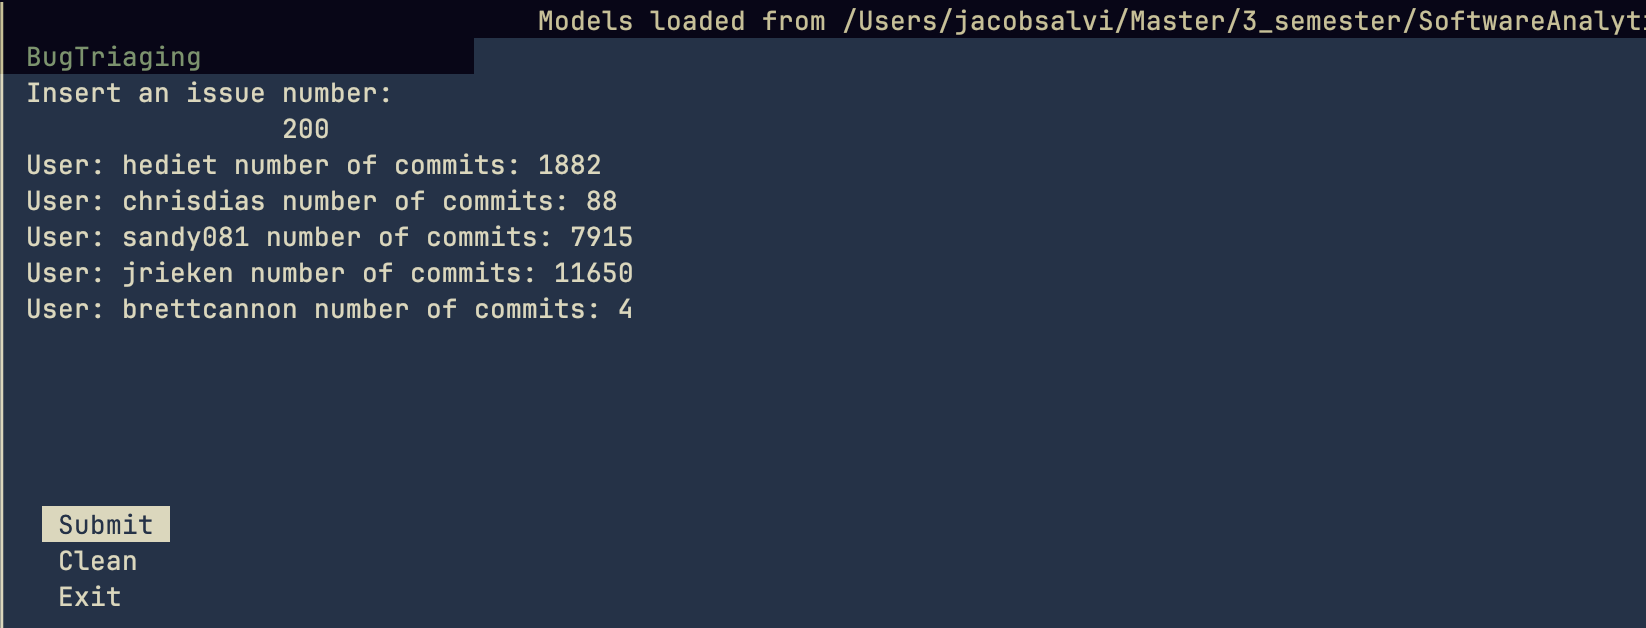
\includegraphics[width=\textwidth]{./tui.png}

To run it is sufficient to run the following code, given that the python environment is set up as described in the README.
\begin{minted}{bash}
python3 src/tui/tui.py
\end{minted}

\section*{Conclusion}
In the project we had the chance of developing a tool for automated bug triaging leveraging using machine learning.\\
Developing this tool we came to appreciate both the strength of such an approach to solve this kind of problem and the challenges faced in developing it.\\
We also appreciated doing this kind of work in a quite realistic context, given that the vscode repository was used, and can picture many practical applications of similar techniques to solve similar challenges in industry.\\
It is also our opinion that we achieved satisfactory results in terms of accuracy.



\end{document}
